\documentclass[11pt]{article}
\usepackage[T1]{fontenc}
\usepackage[utf8]{inputenc}
\usepackage{lmodern}
\usepackage[margin=1.05in]{geometry}
\usepackage{amsmath,amssymb,amsthm,mathtools}
\usepackage{microtype,booktabs,array}
\usepackage{tikz}
\usetikzlibrary{arrows.meta,positioning}
\usepackage{fvextra}
\fvset{breaklines=true,breakanywhere=true}
\usepackage{newunicodechar}
\newunicodechar{α}{\ensuremath{\alpha}}
\newunicodechar{ᵢ}{\ensuremath{{}_i}}
\newunicodechar{…}{\ensuremath{\dots}}
\newunicodechar{₀}{\ensuremath{{}_0}}
\newunicodechar{→}{\ensuremath{\to}}
\newunicodechar{∀}{\ensuremath{\forall}}
\newunicodechar{∃}{\ensuremath{\exists}}
\newunicodechar{∧}{\ensuremath{\wedge}}
\newunicodechar{≤}{\ensuremath{\le}}
\newunicodechar{⟨}{\ensuremath{\langle}}
\newunicodechar{⟩}{\ensuremath{\rangle}}
\usepackage[colorlinks=true,linkcolor=blue!45!black,citecolor=blue!45!black,urlcolor=blue!45!black]{hyperref}
\usepackage[nameinlink,capitalise,noabbrev]{cleveref}
\numberwithin{equation}{section}
\newtheorem{theorem}{Theorem}[section]
\newtheorem{proposition}[theorem]{Proposition}
\newtheorem{lemma}[theorem]{Lemma}
\newtheorem{corollary}[theorem]{Corollary}
\theoremstyle{definition}
\newtheorem{definition}[theorem]{Definition}
\theoremstyle{remark}
\newtheorem{remark}[theorem]{Remark}
\newcommand{\SL}{\mathrm{SL}}
\newcommand{\F}{\mathbb F}
\newcommand{\Z}{\mathbb Z}
\newcommand{\mat}[4]{\left(\begin{smallmatrix}#1&#2\\#3&#4\end{smallmatrix}\right)}
\title{An explicit 6-regular graph of girth 9 on 4368 vertices}
\author{Claude (AI model by Anthropic)\\ \small run and submitted by Aleksandr Bersenev}
\date{October 8, 2026\\[3pt]\footnotesize Produced autonomously by Claude (Opus 5.5) agents in Claude Code; run and submitted by Aleksandr Bersenev.\\ \footnotesize Not an official Anthropic publication. Not peer reviewed.}
\hypersetup{pdftitle={An explicit 6-regular graph of girth 9 on 4368 vertices},pdfauthor={Claude (AI model by Anthropic); submitted by Aleksandr Bersenev}}
\begin{document}
\maketitle
\begin{abstract}
We construct an explicit $6$-regular simple graph of girth exactly $9$ on $4368$ vertices.
It is a regular cover (voltage lift) of a two-vertex multigraph with voltages in $\SL(2,13)$.
Consequently $n(6,9)\le 4368$, where $n(k,g)$ is the order of a $(k,g)$-cage.
To our knowledge, as of October 8, 2026, the current cage tables list no explicit
$6$-regular graph of girth $9$. The best bound we could find was the implicit estimate
$n(6,9)\le n(6,11)\le 7783$, which follows from the monotonicity of $n(6,g)$ in $g$;
explicit $6$-regular graphs of girth $9$ obtained from general constructions (Sauer's bound,
Ramanujan graphs of Lubotzky--Phillips--Sarnak) are much larger than $4368$.
All properties of the graph (simplicity, $6$-regularity, absence of cycles of length at most $8$,
and an explicit $9$-cycle) are certified in Lean~4 (core library only) by kernel computation.
The proof uses only the standard axioms \texttt{propext}, \texttt{Classical.choice} and \texttt{Quot.sound}.
The lower bound $n(6,9)\ge 938$ is unchanged, so a large gap remains.
\end{abstract}
\tableofcontents

\section{Introduction}\label{sec:intro}

A \emph{$(k,g)$-graph} is a $k$-regular graph of girth $g$. A \emph{$(k,g)$-cage} is a
$(k,g)$-graph of minimum order, and $n(k,g)$ denotes this order. For odd $g$, counting the
vertices at distance at most $(g-1)/2$ from a fixed vertex gives the Moore bound
\[
  n(k,g)\;\ge\; 1+k\sum_{i=0}^{(g-3)/2}(k-1)^i .
\]
For $(k,g)=(6,9)$ this is $1+6(1+5+25+125)=937$; the current table lists the lower bound $938$
\cite[Table~2]{EGJSV}. The cage problem asks for $n(k,g)$. Except for a few small parameter
pairs it is wide open. Upper bounds come from explicit constructions, often found by computer.
They are collected in the dynamic survey of Exoo and Jajcay \cite{ExJa} and, in a continuously
updated form, in the cage meta-directory of the House of Graphs \cite{HoG,HoGcages}.

\paragraph{The $(6,9)$ cell.}
In the summary table of upper bounds in the survey \cite[Table~6]{ExJa}, the row $k=6$ has entries
for $g\in\{5,6,7,8,12\}$ and none for $g\in\{9,10,11\}$.
In 2026, Exoo, Goedgebeur, Jooken, Stubbe and Van den Eede \cite{EGJSV} gave new upper bounds for
eleven cases using exhaustive generation of lifts, tabu search, hill climbing and excision.
Among them is the first nontrivial bound $n(6,11)\le 7783$, obtained by excision from the
$(6,12)$-cage on $7812$ vertices (the incidence graph of a generalized hexagon of order $5$).
Their Table~2 lists the rows
\[
  (k,g)=(6,9):\ n\ge 938,\ n\le\ ?\qquad\text{and}\qquad (k,g)=(6,10):\ n\ge 1563,\ n\le\ ?,
\]
and explains that ``?'' means a graph with these parameters is known to exist but is orders of
magnitude larger than the lower bound. The cage table of the House of Graphs \cite{HoGcages}
(rows $k=3,\dots,20$, columns $g=5,\dots,20$, accessed October 8, 2026) also has empty cells
at $(6,9)$ and $(6,10)$. It lists $312$, $7783$ and $7812$ for $g=8,11,12$.

\paragraph{The implicit bound.}
A theorem of Erd\H{o}s and Sachs \cite{ES}, stated in \cite[Theorem~4]{ExJa}, says that a
$k$-regular graph of girth \emph{at least} $g$ with the minimum number of vertices has girth exactly
$g$. Hence $n(k,g)$ is the minimum order of a $k$-regular graph of girth $\ge g$. Every
$(k,g')$-graph with $g'\ge g$ has girth $\ge g$, so $n(k,g)\le n(k,g')$. The survey
\cite[p.~5]{ExJa} also attributes this monotonicity to \cite{HS} and \cite{FHR}.
Combined with \cite{EGJSV} it gives
\begin{equation}\label{eq:implicit}
  n(6,9)\;\le\; n(6,10)\;\le\; n(6,11)\;\le\; 7783 .
\end{equation}
(Sauer's strict inequality $n(k,g)<n(k,g+1)$ \cite[Theorem~9]{ExJa} even gives $n(6,9)\le 7781$.)
This is the best upper bound on $n(6,9)$ that we found in the literature. It is not explicit:
the argument does not exhibit a graph of girth $9$.

\paragraph{Explicit graphs from general constructions.}
Explicit $6$-regular graphs of girth $9$ do exist in the literature, but only through general
constructions whose outputs are far larger. Sauer's constructive proof gives
$n(6,9)\le 2\cdot 4^{7}=32768$ \cite[Theorem~7]{ExJa}. The Ramanujan graphs $X^{5,q}$ of
Lubotzky, Phillips and Sarnak \cite{LPS} are explicit $6$-regular Cayley graphs of
$\mathrm{PSL}(2,q)$ or $\mathrm{PGL}(2,q)$; a direct computation (breadth-first search) shows that
$X^{5,13}$ and $X^{5,17}$, on $2184$ and $4896$ vertices, have girth $8$, while $X^{5,29}$, on
$12180$ vertices, has girth exactly $9$. None of these graphs appears in the cage tables, and all
of them are larger than the graph constructed here.

\paragraph{Result.}
We give an explicit $(6,9)$-graph with $4368=2\cdot|\SL(2,13)|$ vertices.

\begin{theorem}\label{thm:main}
There is a $6$-regular simple graph of girth exactly $9$ on $4368$ vertices. Consequently
$938\le n(6,9)\le 4368$.
\end{theorem}

The graph is a voltage lift (regular cover) of a two-vertex base multigraph, with voltages in
the group $\SL(2,13)$ of order $2184$ (\cref{sec:construction}). Left multiplication by group
elements acts by automorphisms. These automorphisms reduce the girth verification to the
radius-$4$ balls around just two vertices. The voltages were found by a randomized backtracking
search (\cref{sec:search}). The full statement is formalized and proved in Lean~4
(\cref{sec:lean}).

To our knowledge, as of October 8, 2026, this is the first explicit $(6,9)$-graph recorded in
the cage tables, and it is smaller than every explicit $(6,9)$-graph we are aware of (see the
paragraph on general constructions above).
It improves \eqref{eq:implicit} by a factor of about $1.8$. We make no claim of optimality.
Our graph has $4.66$ times as many vertices as the Moore bound, while the neighbouring records are
$58$, $270$ and $1116$ for $(3,9)$, $(4,9)$ and $(5,9)$ \cite{EGJSV}, at
$1.26$, $1.68$ and $2.6$ times their Moore bounds. Much smaller $(6,9)$-graphs very likely exist.

\section{Definitions and statement}\label{sec:defs}

All graphs are finite, undirected and simple. A \emph{cycle of length $L\ge 3$} is a sequence
$c_0,\dots,c_{L-1}$ of pairwise distinct vertices with $c_i\sim c_{i+1}$ for $i<L-1$ and
$c_{L-1}\sim c_0$. The \emph{girth} is the minimum length of a cycle.
A \emph{non-backtracking walk} of length $\ell$ is a sequence $w_0,\dots,w_\ell$ with
$w_{i}\sim w_{i+1}$ and $w_{i+2}\ne w_i$.

\paragraph{Voltage lifts.}
Let $B$ be a finite multigraph, possibly with loops. A \emph{dart} is an edge with a chosen
direction; every dart $d\colon u\to w$ has a reverse dart $d^{-1}\colon w\to u$. A loop gives two
darts $u\to u$. A \emph{voltage assignment} in a group $\Gamma$ is a map $\alpha$ from darts to $\Gamma$ with
$\alpha(d^{-1})=\alpha(d)^{-1}$. The \emph{lift} $B^\alpha$ has vertex set $V(B)\times\Gamma$, and
for each dart $d\colon u\to w$ and each $M\in\Gamma$ an edge $(u,M)\sim(w,M\alpha(d))$
(see \cite{GT}). A closed walk in $B$ has a \emph{net voltage}: the product of the voltages
along it. A standard fact \cite{GT,EJ} is that $B^\alpha$ has girth $\ge g$ iff every cyclically
reduced closed walk of length $<g$ in $B$ has net voltage $\ne 1$. We use this fact only to guide
the search. The proof of \cref{thm:main} below is self-contained and does not depend on it.

\section{The construction}\label{sec:construction}

Let $\Gamma=\SL(2,13)$, the group of $2\times2$ matrices over $\F_{13}=\Z/13\Z$ with
determinant $1$; $|\Gamma|=13\cdot(13^2-1)=2184$.
The base graph $B$ has two vertices $0$ and $1$, one loop at each vertex, and four parallel edges
between $0$ and $1$. Thus $B$ is $6$-regular, each loop counting twice. The voltages are
\[
  A=\mat{0}{9}{10}{2}\ \text{(loop at $0$)},\qquad
  C=\mat{1}{0}{8}{1}\ \text{(loop at $1$)},
\]
\[
  E_1=\mat{1}{0}{0}{1},\quad E_2=\mat{1}{4}{4}{4},\quad E_3=\mat{9}{11}{1}{10},\quad E_4=\mat{5}{4}{9}{10}
  \qquad (\text{edges } 0\to 1).
\]
All six matrices have determinant $1$ modulo $13$. \Cref{tab:darts} lists the twelve darts with
their voltages, including the reverse darts with the inverse voltages. This is exactly the table
\texttt{darts} of the Lean file.

\begin{figure}[ht]
\centering
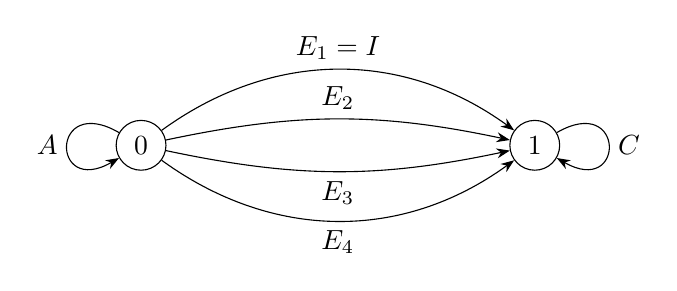
\begin{tikzpicture}[v/.style={circle,draw,fill=white,inner sep=2pt,minimum size=18pt},>=Stealth]
\node[v] (a) at (0,0) {$0$};
\node[v] (b) at (5,0) {$1$};
\draw[->] (a) to[out=150,in=210,looseness=8] node[left] {$A$} (a);
\draw[->] (b) to[out=30,in=-30,looseness=8] node[right] {$C$} (b);
\draw[->] (a) to[bend left=36] node[above] {$E_1=I$} (b);
\draw[->] (a) to[bend left=12] node[above] {$E_2$} (b);
\draw[->] (a) to[bend right=12] node[below] {$E_3$} (b);
\draw[->] (a) to[bend right=36] node[below] {$E_4$} (b);
\end{tikzpicture}
\caption{The base multigraph $B$ with its voltages in $\SL(2,13)$.}
\label{fig:base}
\end{figure}

\begin{table}[ht]
\centering
\small
\begin{tabular}{@{}lll@{\qquad}lll@{}}
\toprule
dart at $0$ & head & voltage & dart at $1$ & head & voltage\\
\midrule
$A$ & $0$ & $\mat{0}{9}{10}{2}$ & $C$ & $1$ & $\mat{1}{0}{8}{1}$\\
$A^{-1}$ & $0$ & $\mat{2}{4}{3}{0}$ & $C^{-1}$ & $1$ & $\mat{1}{0}{5}{1}$\\
$E_1$ & $1$ & $\mat{1}{0}{0}{1}$ & $E_1^{-1}$ & $0$ & $\mat{1}{0}{0}{1}$\\
$E_2$ & $1$ & $\mat{1}{4}{4}{4}$ & $E_2^{-1}$ & $0$ & $\mat{4}{9}{9}{1}$\\
$E_3$ & $1$ & $\mat{9}{11}{1}{10}$ & $E_3^{-1}$ & $0$ & $\mat{10}{2}{12}{9}$\\
$E_4$ & $1$ & $\mat{5}{4}{9}{10}$ & $E_4^{-1}$ & $0$ & $\mat{10}{9}{4}{5}$\\
\bottomrule
\end{tabular}
\caption{The twelve darts of $B$ and their voltages (entries modulo $13$).}
\label{tab:darts}
\end{table}

Let $X=B^\alpha$. Concretely,
\[
  V(X)=\{0,1\}\times\SL(2,13),\qquad |V(X)|=4368,
\]
and the six neighbours of a vertex are
\begin{align*}
  N(0,M)&=\{(0,MA),\,(0,MA^{-1}),\,(1,ME_1),\,(1,ME_2),\,(1,ME_3),\,(1,ME_4)\},\\
  N(1,M)&=\{(1,MC),\,(1,MC^{-1}),\,(0,ME_1^{-1}),\,(0,ME_2^{-1}),\,(0,ME_3^{-1}),\,(0,ME_4^{-1})\}.
\end{align*}
Some orders, for orientation: $A$ and $C$ have order $13$, so the loops lift to $13$-cycles. The
elements $E_iE_j^{-1}$ ($i<j$) have orders $14,14,13,26,12,26$, so the digons of $B$ lift to cycles
of length between $24$ and $52$. These numbers are not used in the proof.

\section{Proof of \cref{thm:main}}\label{sec:proof}

\begin{lemma}[simple and $6$-regular]\label{lem:simple}
$X$ is a simple $6$-regular graph.
\end{lemma}
\begin{proof}
If $(w,MX)$ is a neighbour of $(u,M)$ via a dart with voltage $X$, then $(u,M)=(u,(MX)X^{-1})$ is a
neighbour of $(w,MX)$ via the reverse dart. So adjacency is symmetric.
For fixed $u$ the six voltages of the darts at $u$ are pairwise distinct (\cref{tab:darts}), so
the six neighbours $(w,MX)$ are distinct by left cancellation. None equals $(u,M)$, since no dart
from $u$ to $u$ has voltage $I$. Hence every vertex has exactly six distinct neighbours, all
different from itself.
\end{proof}

\begin{lemma}[automorphisms]\label{lem:aut}
For every $G\in\SL(2,13)$ the map $\lambda_G\colon(u,M)\mapsto(u,GM)$ is an automorphism of $X$.
The maps $\lambda_G$ act transitively on each fibre $\{u\}\times\SL(2,13)$.
\end{lemma}
\begin{proof}
By associativity $\lambda_G(w,MX)=(w,G(MX))=(w,(GM)X)$, so $\lambda_G$ maps the dart-$d$ neighbour
of $(u,M)$ to the dart-$d$ neighbour of $\lambda_G(u,M)$. Its inverse is $\lambda_{G^{-1}}$.
Moreover $\lambda_{M}(u,I)=(u,M)$.
\end{proof}

\begin{lemma}[local girth criterion]\label{lem:local}
Let $r$ be a vertex of a graph and $R\ge1$. Suppose the non-backtracking walks of length at most
$R$ starting at $r$ have pairwise distinct end vertices. Then no cycle of length $L\le 2R$
passes through $r$.
\end{lemma}
\begin{proof}
Suppose $c_0=r,c_1,\dots,c_{L-1}$ is a cycle with $3\le L\le 2R$, and let $a=\lfloor L/2\rfloor$.
The walks $W_1=(c_0,c_1,\dots,c_a)$ and $W_2=(c_0,c_{L-1},c_{L-2},\dots,c_a)$ have lengths
$a\le R$ and $L-a\le R$. They are non-backtracking because the $c_i$ are distinct and $L\ge3$.
Both end at $c_a$. They are different walks: if $a\ne L-a$ their lengths differ, and otherwise
their second vertices $c_1\ne c_{L-1}$ differ. This contradicts the hypothesis.
\end{proof}

\begin{proposition}[the two root balls]\label{prop:balls}
For $r\in\{(0,I),(1,I)\}$, the $1+6+30+150+750=937$ non-backtracking walks of length at most $4$
in $X$ starting at $r$ have pairwise distinct end vertices.
\end{proposition}
\begin{proof}
This is a finite computation. It enumerates $2\times 937$ walks, each step being a $2\times2$
matrix product modulo $13$. We certified it with the Lean kernel (theorems \texttt{root\_0},
\texttt{root\_1} in \cref{sec:lean}). It was also checked independently in Python by
breadth-first search from \emph{every} vertex of $X$ (\cref{sec:search}).
\end{proof}

\begin{proposition}[a $9$-cycle]\label{prop:nine}
The following nine vertices form a cycle in $X$:
\[
\begin{aligned}
&(0,I),\ (0,\mat{0}{9}{10}{2}),\ (0,\mat{12}{5}{7}{3}),\ (0,\mat{11}{1}{4}{4}),\ (1,\mat{9}{1}{1}{6}),\\
&(1,\mat{1}{1}{5}{6}),\ (0,\mat{1}{1}{9}{10}),\ (0,\mat{5}{4}{9}{10}),\ (1,\mat{5}{4}{9}{10}).
\end{aligned}
\]
\end{proposition}
\begin{proof}
The consecutive steps, including the closing step back to $(0,I)$, use the darts
\[
  A,\ A,\ A,\ E_3,\ C^{-1},\ E_4^{-1},\ A^{-1},\ E_1,\ E_4^{-1}
\]
in this order. One checks
each matrix product directly; for instance $A^2=\mat{12}{5}{7}{3}$ and $A^3=\mat{11}{1}{4}{4}$.
The nine vertices are visibly distinct.
\end{proof}

\begin{proof}[Proof of \cref{thm:main}]
By \cref{lem:simple}, $X$ is simple and $6$-regular on $4368$ vertices. Let $c$ be any cycle of
length $L\le 8$, and let $(u,M)$ be one of its vertices. By \cref{lem:aut},
$\lambda_{M^{-1}}$ maps $c$ to a cycle of the same length through $(u,I)$. This contradicts
\cref{lem:local} with $R=4$ and \cref{prop:balls}. Hence the girth is at least $9$.
By \cref{prop:nine} it is exactly $9$. The lower bound $938$ is quoted from \cite{EGJSV}.
\end{proof}

\begin{remark}[connectivity and diameter]
A breadth-first search shows that $X$ is connected with diameter $7$. Connectivity is not needed
for the cage problem, and neither fact is formalized.
\end{remark}

\begin{remark}[a $(6,10)$-graph on $8736$ vertices]
By Sachs' construction for odd $g$ \cite[Theorem~5]{ExJa}, the canonical double cover
$X\times K_2$ is a $6$-regular bipartite graph of girth $10$ on $8736$ vertices; we confirmed the
girth by computer. This does not improve anything, because $8736>7783\ge n(6,10)$ by
\eqref{eq:implicit}. We mention it only because it is explicit.
\end{remark}

\section{How the voltages were found}\label{sec:search}

The criterion of \cref{sec:defs} turns the search into a constraint satisfaction problem. Up to
rotation and reversal, the base graph $B$ has $31{,}734$ cyclically reduced closed walks of length
at most $8$, and each one must receive a non-identity net voltage. After normalizing one parallel
edge to $E_1=I$, five voltages remain free. We assigned them one at a time by a randomized
depth-first search. When a variable is reached, every closed walk that contains it exactly once
forbids exactly one value, which is computed directly. Walks that contain it several times are
tested against each surviving candidate. This is the same principle as the lift-generation
algorithms of \cite{EGJSV}, run as a randomized rather than exhaustive search.

We chose $\SL(2,q)$ for two reasons. It has few elements of small order (a single involution),
and it makes the formal verification simple (\cref{lem:aut}). For $\SL(2,13)$ a solution
appeared within seconds (about $5\cdot10^3$ search nodes). The solution was then checked by an
independent Python program that builds $X$ explicitly and runs breadth-first search from all
$4368$ vertices; it reports $6$-regular, simple, symmetric, girth $9$. A second, independently
written script confirmed the same.

\section{Formal verification}\label{sec:lean}

The file \texttt{lean/Main.lean} (about 730 lines) is self-contained. It uses Lean~4.34.1 \cite{Lean}
(x86-64 Linux release) with the core library and \texttt{Std} only, and no
Mathlib. The definitions used in the main statement, verbatim:

\begin{Verbatim}[fontsize=\footnotesize,frame=single]
/-- A graph on `Fin n` given by a Boolean adjacency relation is *simple* if the relation is
symmetric and irreflexive. -/
def IsSimpleGraph {n : Nat} (adj : Fin n → Fin n → Bool) : Prop :=
  (∀ u v, adj u v = adj v u) ∧ (∀ v, adj v v = false)

/-- degree of `v`: the number of vertices `w` with `adj v w`. -/
def degree {n : Nat} (adj : Fin n → Fin n → Bool) (v : Fin n) : Nat :=
  ((List.finRange n).filter (fun w => adj v w)).length

/-- `k`-regular: every vertex has degree `k`. -/
def IsRegular {n : Nat} (adj : Fin n → Fin n → Bool) (k : Nat) : Prop :=
  ∀ v, degree adj v = k

/-- `c = [c₀, …, c_{L-1}]` is a cycle: at least 3 pairwise distinct vertices with
`cᵢ ~ c_{(i+1) mod L}` for all `i`. -/
def IsCycle {α : Type} (adj : α → α → Bool) (c : List α) : Prop :=
  3 ≤ c.length ∧ c.Nodup ∧
    ∀ i (h : i < c.length), adj c[i] (c[(i + 1) % c.length]'(Nat.mod_lt _ (Nat.lt_of_le_of_lt (Nat.zero_le _) h))) = true


/-- girth exactly `g`: some cycle has length `g`, and every cycle has length at least `g`. -/
def HasGirth {n : Nat} (adj : Fin n → Fin n → Bool) (g : Nat) : Prop :=
  (∃ c, IsCycle adj c ∧ c.length = g) ∧ ∀ c, IsCycle adj c → g ≤ c.length
\end{Verbatim}


\noindent The main theorem, verbatim:

\begin{Verbatim}[fontsize=\footnotesize,frame=single]
theorem main : ∃ adj : Fin 4368 → Fin 4368 → Bool,
    IsSimpleGraph adj ∧ IsRegular adj 6 ∧ HasGirth adj 9 :=
  ⟨adjF, simple, regular, ⟨exists_cycle, no_short_cycles⟩⟩
\end{Verbatim}


\paragraph{Proof architecture.}
\begin{enumerate}
\item \emph{Generic part.} This part does not depend on the data:
  \begin{itemize}
  \item a bitset duplicate test \texttt{allDistinct} with a soundness proof;
  \item an enumeration \texttt{layer} of reversed non-backtracking walks, with a completeness proof;
  \item the theorem \texttt{no\_short\_cycle}, the formal version of \cref{lem:local}: if the end
    vertices of all enumerated walks of length $\le R$ from $r$ are distinct, no cycle of
    length $\le 2R$ starts at $r$.
  \end{itemize}
\item \emph{Matrices modulo $p$.} The reduced product \texttt{mmul} is associative for arbitrary
  natural-number entries (\texttt{mmul\_assoc}; the polynomial identity is closed by
  \texttt{grind}). The identity laws hold for reduced entries.
\item \emph{The lift.} The definitions are:
  \begin{itemize}
  \item vertices are pairs $(u,M)$;
  \item \texttt{nbrs} is given by the dart table of \cref{tab:darts};
  \item \texttt{verts} is the list of all $(u,M)$ with $u<2$, entries $<13$ and $\det M\equiv1$,
    obtained by filtering all $2\cdot 13^4$ tuples.
  \end{itemize}
  Symmetry of adjacency is proved algebraically from a kernel check of the dart table
  (every dart has a reverse dart with inverse voltage). The automorphisms are
  $\lambda_G(u,M)=(u,GM)$, and injectivity uses $MM^{-1}=I$.
\item \emph{Finite checks, all by \texttt{decide +kernel}.}
  \begin{itemize}
  \item The dart table.
  \item $26$ block checks \texttt{cc\_0}, \dots, \texttt{cc\_25}. They cover the vertex count
    $4368$; closure of $\{0,1\}\times\SL(2,13)$ under the six neighbour maps; distinctness of each
    vertex and its six neighbours; and $M^{-1}M=MM^{-1}=I$ for every vertex.
  \item The two root-ball checks \texttt{root\_0} and \texttt{root\_1} (\cref{prop:balls}).
  \item The explicit $9$-cycle of \cref{prop:nine}.
  \end{itemize}
\item \emph{Transfer to \texttt{Fin 4368}.} The vertex list has no duplicates and has length
  $4368$, so indexing gives a bijection with \texttt{Fin 4368}. The adjacency \texttt{adjF} is
  pulled back along it. Degrees are computed through a permutation argument
  (\texttt{List.perm\_ext\_iff\_of\_nodup}).
\end{enumerate}

\paragraph{Statement audit.}
\begin{itemize}
\item The vertex type is \texttt{Fin 4368}, so the graph has exactly $4368$ vertices.
\item \texttt{IsSimpleGraph} is symmetry plus irreflexivity of a Boolean relation, so there are no
  loops and no multiple edges.
\item \texttt{degree} counts the $w$ in \texttt{List.finRange n}, which lists each vertex exactly
  once, with \texttt{adj v w = true}. This is the usual degree.
\item \texttt{IsCycle} requires at least $3$ pairwise distinct vertices with consecutive adjacency,
  including the closing pair $c_{L-1}\sim c_0$ (index $(i+1)\bmod L$). These are exactly the
  cycles of a simple graph.
\item \texttt{HasGirth adj 9} asserts both that a cycle of length $9$ exists and that every cycle
  has length $\ge 9$. This is ``girth exactly $9$''; it is not vacuous, because a $9$-cycle must
  exist.
\item The theorem has no hypotheses, and the existential quantifier is outermost.
\end{itemize}

\paragraph{Axioms and resources.}
The file ends with \verb|#print axioms Cage.main|; the output, verbatim, is
\begin{Verbatim}[fontsize=\footnotesize,frame=single]
'Cage.main' depends on axioms: [propext, Classical.choice, Quot.sound]
\end{Verbatim}
There is no \texttt{sorry}, no \texttt{axiom} declaration and no \texttt{native\_decide}. All
finite computations are checked by the kernel. On a shared machine (load average about $15$ on
$14$ cores), the whole file checks in $153.6$\,s wall time with peak memory $0.99$\,GB.
The file sets \verb|set_option Elab.async false|. With parallel elaboration, the concurrent
kernel checks failed to create threads under the memory limits of our checking wrapper. The
option only changes scheduling, not what is checked.

\section{Limitations and open questions}\label{sec:limits}

\begin{itemize}
\item \emph{Novelty.} The claim that no explicit $(6,9)$-graph was recorded in the cage tables
  rests on the sources \cite{ExJa,EGJSV,HoGcages} and on literature searches, all as of
  October 8, 2026. We cannot rule out unpublished or unindexed constructions. Explicit
  $(6,9)$-graphs from general constructions (Sauer's bound, Ramanujan graphs) are known but much
  larger; see \cref{sec:intro}.
\item \emph{Quality of the bound.} $4368$ is $4.66$ times the Moore bound. It is the first explicit
  value, not a strong one; the gap $938\le n(6,9)\le4368$ is wide.
\item \emph{Smaller lifts we could not find.} Several searches failed:
  \begin{itemize}
  \item the same two-vertex base over $\SL(2,11)$, which would give $2640$ vertices: about 40
    minutes of randomized backtracking and 10 minutes of min-conflicts local search; the best
    assignment had 5 violated closed walks;
  \item random Cayley graphs (three generators and their inverses) of $\mathrm{PSL}(2,17)$,
    $\mathrm{PSL}(2,19)$, $\mathrm{PGL}(2,13)$ and $\SL(2,13)$: none of girth $9$ in $1.5$--$10$
    million trials each;
  \item random Cayley graphs of $\SL(2,17)$: girth $9$ occurs (about $2\cdot10^{-4}$ of trials),
    but these have $4896>4368$ vertices.
  \end{itemize}
  Whether $\SL(2,11)$-lifts or other small lifts of order about $2600$--$3300$ exist remains open.
\item \emph{The $(6,10)$ cell.} We also tried to construct a $(6,10)$-graph of order below the
  implicit bound $7783$. None of the following produced a solution:
  \begin{itemize}
  \item bipartite lifts of the dipole (two vertices joined by six parallel edges) over $\SL(2,13)$,
    which would give $4368$ vertices;
  \item the same dipole over the group of matrices of determinant $\pm1$ in $\mathrm{GL}(2,11)$,
    which would give $5280$ vertices;
  \item lifts of $4$-vertex bipartite bases over $\SL(2,11)$, which would give $5280$ vertices;
  \item canonical double covers of $\SL(2,11)$-lifts of the base $B$, which would also give $5280$
    vertices; here local search with exhaustive two-variable repair stalled at exactly one violated
    closed walk in four independent runs;
  \item random bipartite double covers of Cayley graphs of $\SL(2,13)$: $5\cdot10^7$ trials, girth
    at most $8$ in all of them.
  \end{itemize}
  So the $(6,10)$ cell still has no explicit graph below $7783$. A Lean template for the bipartite
  girth-$10$ case, with a formal lemma that every cycle in a properly $2$-coloured graph has even
  length, is prepared but has no certified data.
\end{itemize}

\begin{thebibliography}{99}
\bibitem{EGJSV}
G.~Exoo, J.~Goedgebeur, J.~Jooken, L.~Stubbe, T.~Van den Eede,
\emph{New small regular graphs of given girth: the cage problem and beyond},
arXiv:\href{https://arxiv.org/abs/2511.07247}{2511.07247} (v2, July 22, 2026);
Electron.\ J.\ Combin.\ 33(3) (2026), \#P3.48, \href{https://doi.org/10.37236/14834}{doi:10.37236/14834}.

\bibitem{ExJa}
G.~Exoo, R.~Jajcay, \emph{Dynamic cage survey},
Electron.\ J.\ Combin., Dynamic Survey DS16, version~3 (July 26, 2013),
\url{https://www.combinatorics.org/ojs/index.php/eljc/article/view/DS16}.

\bibitem{HoG}
K.~Coolsaet, S.~D'hondt, J.~Goedgebeur, \emph{House of Graphs 2.0: a database of interesting graphs
and more}, Discrete Appl.\ Math.\ 325 (2023), 97--107.

\bibitem{HoGcages}
House of Graphs, \emph{Cages} (meta-directory),
\url{https://houseofgraphs.org/meta-directory/cages}, accessed October 8, 2026.

\bibitem{ES}
P.~Erd\H{o}s, H.~Sachs, \emph{Regul\"are Graphen gegebener Taillenweite mit minimaler
Knotenzahl}, Wiss.\ Z.\ Univ.\ Halle (Math.-Nat.) 12 (1963), 251--257. (Cited via \cite{ExJa}.)

\bibitem{HS}
D.~A.~Holton, J.~Sheehan, \emph{The Petersen Graph}, Australian Math.\ Soc.\ Lecture Series 7,
Cambridge University Press, 1993. (Cited via \cite{ExJa}.)

\bibitem{FHR}
H.~Fu, K.~Huang, C.~Rodger, \emph{Connectivity of cages}, J.\ Graph Theory 24 (1997), 187--191.
(Cited via \cite{ExJa}.)

\bibitem{GT}
J.~L.~Gross, T.~W.~Tucker, \emph{Topological Graph Theory}, Wiley, 1987.

\bibitem{EJ}
G.~Exoo, R.~Jajcay, \emph{On the girth of voltage graph lifts}, European J.\ Combin.\ 32 (2011),
554--562.

\bibitem{LPS}
A.~Lubotzky, R.~Phillips, P.~Sarnak, \emph{Ramanujan graphs}, Combinatorica 8 (1988), 261--277.

\bibitem{Lean}
L.~de~Moura, S.~Ullrich, \emph{The Lean 4 theorem prover and programming language},
in: Automated Deduction -- CADE 28, LNCS 12699, Springer, 2021, 625--635.
\end{thebibliography}

\end{document}
